% Slide deck documenting the jet clustering algorithms used in FCCJetBenchmarks.
%
% Companion to the prose note doc/jet_algorithms.tex; this file is the
% presentation form (comparison tables + schematics), not a rewrite of it.
%
% Build:  pdflatex clustering_algorithms_slides.tex
\documentclass[aspectratio=169,10pt]{beamer}

\usetheme{default}
\usepackage[T1]{fontenc}
\usepackage{amsmath}
\usepackage{amssymb}
\usepackage{booktabs}
\usepackage{tikz}
\usetikzlibrary{arrows.meta,positioning}

\setbeamertemplate{navigation symbols}{}
\setbeamertemplate{itemize items}[circle]
\setbeamertemplate{blocks}[rounded][shadow=false]
\setbeamerfont{frametitle}{series=\bfseries,size=\large}
\setbeamerfont{framesubtitle}{size=\small,shape=\itshape}

% ---------------------------------------------------------------- palette ----
% Matches the figure conventions used by src/plotting/*.
\definecolor{pfblue}{HTML}{1F77B4}     % Durham / PFJets
\definecolor{caviolet}{HTML}{7A3CBF}   % ee Cambridge/Aachen, p = 0
\definecolor{ktamber}{HTML}{D18B00}    % ee kT, p = +1
\definecolor{aktteal}{HTML}{2A9D8F}    % ee anti-kT, p = -1
\definecolor{calogreen}{HTML}{2CA02C}  % CaloJets
\definecolor{inkgrey}{HTML}{3A3A3A}
% Darker shade of the same amber, used only for small text so that the contrast
% against the white background stays adequate.
\definecolor{ktamberink}{HTML}{9A6700}

\setbeamercolor{structure}{fg=pfblue}
\setbeamercolor{frametitle}{fg=pfblue}
\setbeamercolor{normal text}{fg=inkgrey}
\setbeamercolor{alerted text}{fg=caviolet}
\setbeamercolor{block title}{fg=white,bg=pfblue}
\setbeamercolor{block body}{bg=pfblue!6}

\newcommand{\ee}{$e^{+}e^{-}$}
\newcommand{\dij}{d_{ij}}
\newcommand{\diB}{d_{iB}}
\newcommand{\Cdur}[1]{\textcolor{pfblue}{#1}}
\newcommand{\Cca}[1]{\textcolor{caviolet}{#1}}
\newcommand{\Ckt}[1]{\textcolor{ktamberink}{#1}}
\newcommand{\Cakt}[1]{\textcolor{aktteal}{#1}}
\newcommand{\Ccalo}[1]{\textcolor{calogreen}{#1}}
% One panel of the "which pair merges first" schematic. Defined here rather than
% in the frame body: a beamer frame cannot contain a macro definition using #.
%   #1 x offset   #2 colour   #3 title   #4 the pair that merges first
\newcommand{\mergepanel}[4]{%
  \begin{scope}[xshift=#1]
    % Geometry chosen so that the three exponents genuinely pick three
    % different pairs (verified numerically with E_H=4, E_M=1, E_S=0.22):
    %   p=-1  H-Ma   (hardest particle takes its nearest neighbour)
    %   p= 0  Ma-Mb  (globally smallest angle)
    %   p=+1  Mb-S   (softest particle taken first, by the medium nearest it)
    % Margins over the runner-up pair are x2.2, x4.1 and x1.7 respectively.
    \coordinate (H)  at (-1.05,0.20);
    \coordinate (Ma) at (-0.35,0.78);
    \coordinate (Mb) at (0.05,0.98);
    \coordinate (S)  at (1.02,0.50);
    \draw[#2,line width=2.6pt,opacity=0.40] #4;
    \fill[#2] (H) circle (7.5pt);
    \fill[#2!72] (Ma) circle (4.4pt);
    \fill[#2!72] (Mb) circle (4.4pt);
    \fill[#2!48] (S) circle (2.4pt);
    \node[inkgrey,font=\scriptsize,left=9pt of H]   {$H$};
    \node[inkgrey,font=\scriptsize,left=6pt of Ma]  {$M$};
    \node[inkgrey,font=\scriptsize,above=6pt of Mb] {$M$};
    \node[inkgrey,font=\scriptsize,right=5pt of S]  {$S$};
    \node[#2,anchor=south] at (-0.2,1.60) {\textbf{#3}};
  \end{scope}}

\title{Jet clustering algorithms in the FCC jet benchmarks}
\subtitle{Distance measures, termination rules, and what the method directories contain}
\author{FCCJetBenchmarks}
\date{\today}

\begin{document}

\begin{frame}[plain]
  \titlepage
  \begin{center}\footnotesize
    Colour coding follows the repository figures:\\[4pt]
    \textcolor{pfblue}{$\blacksquare$}\,Durham / PFJets \quad
    \textcolor{caviolet}{$\blacksquare$}\,\ee{} C/A, $p=0$ \quad
    \textcolor{ktamberink}{$\blacksquare$}\,\ee{} $k_T$, $p=+1$ \quad
    \textcolor{aktteal}{$\blacksquare$}\,\ee{} anti-$k_T$, $p=-1$ \quad
    \textcolor{calogreen}{$\blacksquare$}\,CaloJets
  \end{center}
\end{frame}

% ============================================================== common setup =
\begin{frame}{Common framework}
  \framesubtitle{All jets are built with FastJet through the FCCAnalyses \texttt{JetClustering} functors}

  Every algorithm below is a sequential recombination algorithm: take the
  smallest of all $\dij$ and $\diB$, merge the pair $ij$ or declare $i$ a jet,
  repeat. The algorithms differ only in the distance measure and in the
  termination rule.

  \medskip
  \begin{center}
  \small
  \begin{tabular}{@{}ll@{}}
    \toprule
    Setting & Value \\
    \midrule
    Collision & \ee{} at $\sqrt{s} = 240$\,GeV, $ZH$ production \\
    Recombination scheme & $E$-scheme, four-momenta added \\
    Gen-jet input & stable generator particles, neutrinos removed \\
    Reco-jet input & particle-flow objects \\
    Acceptance & $|\eta| < 2.56$ \\
    Radius grid & $R = 0.4,\ 0.6,\ 0.8,\ 1.0,\ 1.2,\ 1.4$ \\
    Jets per process & $N = 2,\ 4$ or $6$ \\
    \bottomrule
  \end{tabular}
  \end{center}

  \medskip
  The radius grid and $N$ are defined by \texttt{RADIUS\_SCAN} and
  \texttt{NUMBER\_OF\_JETS} in \texttt{src/process\_config.py}.
\end{frame}

% =========================================================== measure compare =
\begin{frame}{Distance measures side by side}

  \begin{center}
  \renewcommand{\arraystretch}{2.0}
  \small
  \begin{tabular}{@{}lccl@{}}
    \toprule
    Algorithm & $\dij$ & $\diB$ & Termination \\
    \midrule
    generalized \ee{} $k_T$
      & $\min\!\left(E_i^{2p}, E_j^{2p}\right)\dfrac{1-\cos\theta_{ij}}{1-\cos R}$
      & $E_i^{2p}$
      & inclusive \\
    \addlinespace[0.7ex]
    \Cdur{Durham} (\ee{} $k_T$)
      & $\dfrac{2\min\!\left(E_i^{2}, E_j^{2}\right)(1-\cos\theta_{ij})}{E_{\mathrm{vis}}^{2}}$
      & ---
      & exclusive, exactly $N$ \\
    \addlinespace[0.7ex]
    hadron-collider anti-$k_T$
      & $\min\!\left(p_{T,i}^{-2}, p_{T,j}^{-2}\right)\dfrac{\Delta R_{ij}^{2}}{R^{2}}$
      & $p_{T,i}^{-2}$
      & inclusive \\
    \bottomrule
  \end{tabular}

  \medskip
  {\small Specialisations of the first row:
   \Cakt{$p=-1$, anti-$k_T$} \quad
   \Cca{$p=0$, C/A} \quad
   \Ckt{$p=+1$, $k_T$}}
  \end{center}

  \smallskip
  The \ee{} measures use angular, not rapidity, distances: at a lepton collider
  there is no beam remnant to be boosted along. The hadron-collider measure is
  reachable via \texttt{-{}-jet-algorithm AK} and is kept for cross-checks
  only; it enters no production figure.
\end{frame}

% ================================================================ exponent p =
\begin{frame}{The exponent \texorpdfstring{$p$}{p} selects the algorithm}
  \framesubtitle{FastJet \texttt{ee\_genkt\_algorithm}; sixth argument of \texttt{clustering\_ee\_genkt}}

  \begin{center}
  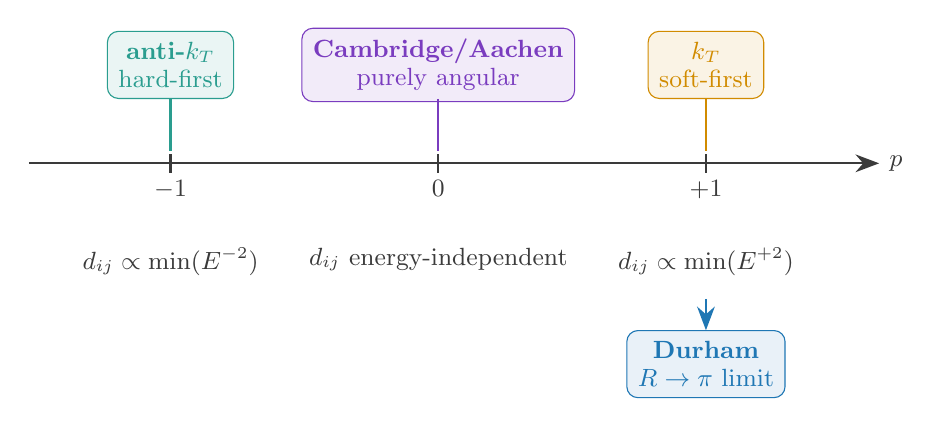
\begin{tikzpicture}[>={Stealth[length=3mm]},font=\small]
    % axis
    \draw[->,thick,inkgrey] (-5.2,0) -- (5.6,0) node[right,inkgrey] {$p$};
    \foreach \x/\lab in {-3.4/$-1$, 0/$0$, 3.4/$+1$}
      \draw[thick,inkgrey] (\x,-0.12) -- (\x,0.12) node[below=6pt] {\lab};

    % algorithm nodes
    \node[aktteal,  fill=aktteal!10,  draw=aktteal,  rounded corners, inner sep=4pt,
          align=center] at (-3.4,1.25) {\textbf{anti-$k_T$}\\[-1pt] hard-first};
    \node[caviolet, fill=caviolet!10, draw=caviolet, rounded corners, inner sep=4pt,
          align=center] at (0,1.25)    {\textbf{Cambridge/Aachen}\\[-1pt] purely angular};
    \node[ktamber,  fill=ktamber!10,  draw=ktamber,  rounded corners, inner sep=4pt,
          align=center] at (3.4,1.25)  {\textbf{$k_T$}\\[-1pt] soft-first};

    \draw[aktteal,thick]  (-3.4,0.82) -- (-3.4,0.16);
    \draw[caviolet,thick] (0,0.82)    -- (0,0.16);
    \draw[ktamber,thick]  (3.4,0.82)  -- (3.4,0.16);

    % energy weighting annotation
    \node[anchor=north,inkgrey] at (-3.4,-0.95) {$\dij \propto \min(E^{-2})$};
    \node[anchor=north,inkgrey] at (0,-0.95)    {$\dij$ energy-independent};
    \node[anchor=north,inkgrey] at (3.4,-0.95)  {$\dij \propto \min(E^{+2})$};

    % Durham limit
    \node[pfblue,fill=pfblue!10,draw=pfblue,rounded corners,inner sep=4pt,
          align=center] at (3.4,-2.55) {\textbf{Durham}\\[-1pt] $R \to \pi$ limit};
    \draw[pfblue,thick,->] (3.4,-1.72) -- (3.4,-2.12);
  \end{tikzpicture}
  \end{center}

  \smallskip
  Method directories: \Cakt{\texttt{PF\_EEAntiKtR*}} ($p=-1$),
  \Cca{\texttt{PF\_EECambridgeR*}} ($p=0$),
  \Ckt{\texttt{PF\_EEKtR*}} ($p=+1$), each spanning the six radii.
\end{frame}

% ============================================================ merging order ==
\begin{frame}{Which pair merges first}
  \framesubtitle{Identical configuration in all three panels; marker size indicates energy}

  \begin{center}
  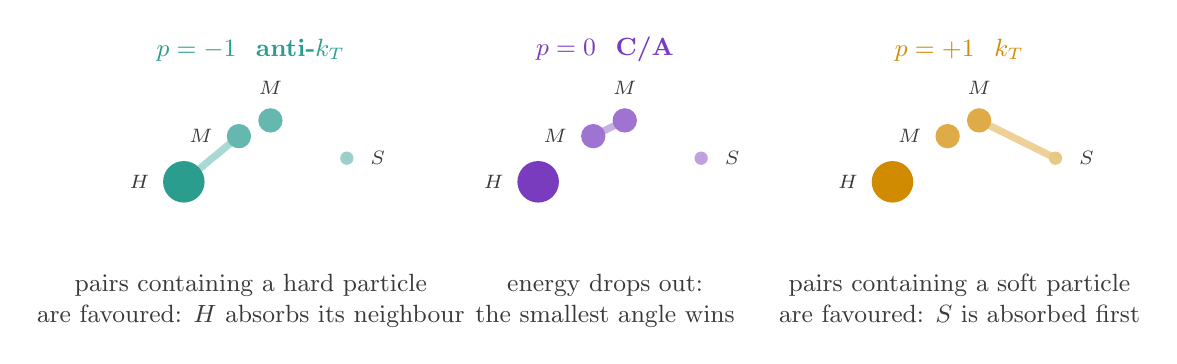
\begin{tikzpicture}[font=\small]
    % One hard (H), two medium (M) closest to each other, one soft (S) out by
    % the right-hand M. The three exponents then select three different pairs.
    \mergepanel{-4.5cm}{aktteal}{$p = -1$\ \ anti-$k_T$}{(H) -- (Ma)}
    \mergepanel{0cm}{caviolet}{$p = 0$\ \ C/A}{(Ma) -- (Mb)}
    \mergepanel{4.5cm}{ktamber}{$p = +1$\ \ $k_T$}{(Mb) -- (S)}

    \node[inkgrey,anchor=north,align=center] at (-4.7,-0.85)
      {pairs containing a hard particle\\ are favoured: $H$ absorbs its neighbour};
    \node[inkgrey,anchor=north,align=center] at (-0.2,-0.85)
      {energy drops out:\\ the smallest angle wins};
    \node[inkgrey,anchor=north,align=center] at (4.3,-0.85)
      {pairs containing a soft particle\\ are favoured: $S$ is absorbed first};
  \end{tikzpicture}
  \end{center}

  \smallskip
  The weight $\min(E_i^{2p},E_j^{2p})$ reorders the pairs at fixed geometry, so
  $p$ fixes the merge sequence and thereby the jet substructure.
\end{frame}

% ============================================================ R dependence ===
\begin{frame}{Two consequences of the \texorpdfstring{\ee{}}{ee} measure}

  \begin{block}{$R$ acts only on the beam comparison}
    \begin{itemize}
      \item $1/(1-\cos R)$ is a global constant and never reorders the $\dij$
            among themselves.
      \item The whole $R$ dependence enters through $\dij$ versus $\diB$, i.e.\
            through which particles are split off rather than merged.
      \item Small $R$ therefore yields more, narrower jets.
    \end{itemize}
  \end{block}

  \begin{block}{$p = +1$ degenerates into Durham}
    \begin{itemize}
      \item As $R \to \pi$ the beam term can no longer win.
            \texttt{JetDefinition.hh} states that $R > 2$ with $p = 1$ gives
            \texttt{ee\_kt}.
      \item Measured on simulated 6-jet events: exclusive-to-$N$ clustering with
            $p = +1$ is bit-identical to Durham for $R \gtrsim 0.6$.
      \item Consequence: the $k_T$ family is run \emph{inclusively}, where $R$
            genuinely changes the jets. An exclusive scan would reproduce
            \Cdur{\texttt{PF\_Durham}}.
    \end{itemize}
  \end{block}
\end{frame}

% ====================================================== not-clustering steps =
\begin{frame}{Two entries that are not clustering algorithms}

  \begin{block}{CaloJets --- the no-particle-flow reference}
    Jets are read from the \texttt{CaloJetDurham} branch produced by Delphes,
    which applies Durham to calorimeter towers rather than to particle-flow
    objects. No clustering is performed in this framework. Method directory
    \Ccalo{\texttt{CaloJets\_Durham}}.
  \end{block}

  \begin{block}{Energy recovery --- the ``-ER'' variants}
    A post-processing step on the inclusive C/A output
    (\texttt{ZHfunctions::energy\_recovery},
    \texttt{src/histmaker\_functions/functions.h}). The $N$ leading jets are
    kept and every surplus jet is recombined into them, so the event ends with
    exactly $N$ jets. Available for all three exponents.

    \smallskip
    It acts only where the clustering overproduces, so its size is governed by
    $N$. At $R = 0.4$ on $Z(\to\nu\nu)H(\to qq)$ ($N = 2$) it moves the $m_H$
    peak from $119.9$ to $124.9$~GeV and renders the result independent of both
    radius and exponent, the $N$ jets then holding every visible particle. On
    the 6-jet light-flavour process at $R \ge 0.8$ the clustering already yields
    $\le N$ jets and energy recovery is the identity.
  \end{block}
\end{frame}

% ======================================================== directory mapping ==
\begin{frame}{Method directories}

  \begin{center}
  \footnotesize
  \begin{tabular}{@{}l@{\hspace{2.2em}}l@{\hspace{1.6em}}c@{\hspace{1.6em}}l@{}}
    \toprule
    Method directory & FastJet & $p$ & Mode \\
    \midrule
    \Cdur{\texttt{PF\_Durham}}                        & \texttt{ee\_kt}            & $+1$ & exclusive, $N$ jets \\
    \Ccalo{\texttt{CaloJets\_Durham}}                 & \texttt{ee\_kt} (Delphes)  & $+1$ & exclusive; calorimeter towers \\
    \Cdur{\texttt{PF\_Durham\_IdealMatching}}         & \texttt{ee\_kt}            & $+1$ & exclusive; PFlow-replaced constituents \\
    \Cca{\texttt{PF\_EECambridgeR\{04..14\}}}         & \texttt{ee\_genkt}         & $0$  & inclusive \\
    \Cca{\texttt{PF\_E\_recovery\_EECambridgeR\{04..14\}}} & \texttt{ee\_genkt}    & $0$  & inclusive $+$ energy recovery \\
    \Ckt{\texttt{PF\_EEKtR\{04..14\}}}                & \texttt{ee\_genkt}         & $+1$ & inclusive \\
    \Cakt{\texttt{PF\_EEAntiKtR\{04..14\}}}           & \texttt{ee\_genkt}         & $-1$ & inclusive \\
    \bottomrule
  \end{tabular}
  \end{center}

  \medskip
  The Durham call is
  \texttt{JetClustering::clustering\_ee\_kt(2, N, 1, 0)}, with
  \texttt{exclusive}${}=2$ meaning ``exactly \texttt{cut} jets'' and
  $E$-ordered output.
\end{frame}

% =========================================================== measured rates =
\begin{frame}{Measured behaviour at \texorpdfstring{$R = 0.8$}{R = 0.8}}
  \framesubtitle{$Z(\to q\bar{q})\,H(\to WW \to q\bar{q}q\bar{q})$, six expected jets}

  \begin{center}
  \small
  \begin{tabular}{@{}lcc@{}}
    \toprule
    Algorithm & Events yielding 6 jets & Fully-matched-event pass rate \\
    \midrule
    \Ckt{\ee{} $k_T$ ($p=+1$)}            & 74\% & 0.61 \\
    \Cca{\ee{} C/A ($p=0$)}               & 98\% & 0.82 \\
    \Cdur{Durham (exclusive)}             & ---  & 0.87 \\
    \bottomrule
  \end{tabular}
  \end{center}

  \medskip
  \begin{itemize}
    \item At equal $R$, $k_T$ merges considerably more aggressively than C/A,
          and the lost jets propagate into the matching efficiency.
    \item Durham imposes $N$, so it has no jet-multiplicity distribution and no
          radius to scan.
  \end{itemize}
\end{frame}

% ======================================================= naming correction ===
\begin{frame}{Naming correction, 2026-09}
  \framesubtitle{Required for reading any earlier figure or table}

  Until 2026-09 the $p = 0$ scan was labelled ``generalized \ee{} anti-$k_T$''
  and its directories were named \texttt{PF\_AntiKtR*}. That label was wrong.
  The code called

  \begin{center}
    \texttt{clustering\_ee\_genkt(R, 0, 0, 0)}
  \end{center}

  with four arguments, whereas the signature is

  \begin{center}
    \texttt{(radius, exclusive, cut, sorted, recombination=0, exponent=0.)}
  \end{center}

  The exponent defaulted to $0$, so those runs were \Cca{Cambridge/Aachen} and
  never anti-$k_T$.

  \medskip
  \begin{itemize}
    \item The histograms are valid C/A data; they were relabelled rather than
          re-run. Directories are now \Cca{\texttt{PF\_EECambridgeR*}}.
    \item Genuine \ee{} anti-$k_T$ ($p = -1$) is being run for the first time
          now, as \Cakt{\texttt{PF\_EEAntiKtR*}}.
    \item Any older figure showing ``ee-AK'', ``anti-kt'' or \texttt{AntiKtR}
          must be read as Cambridge/Aachen.
  \end{itemize}
\end{frame}

\end{document}
